% Created by tikzDevice version 0.12.6 on 2024-07-05 15:51:11
% !TEX encoding = UTF-8 Unicode
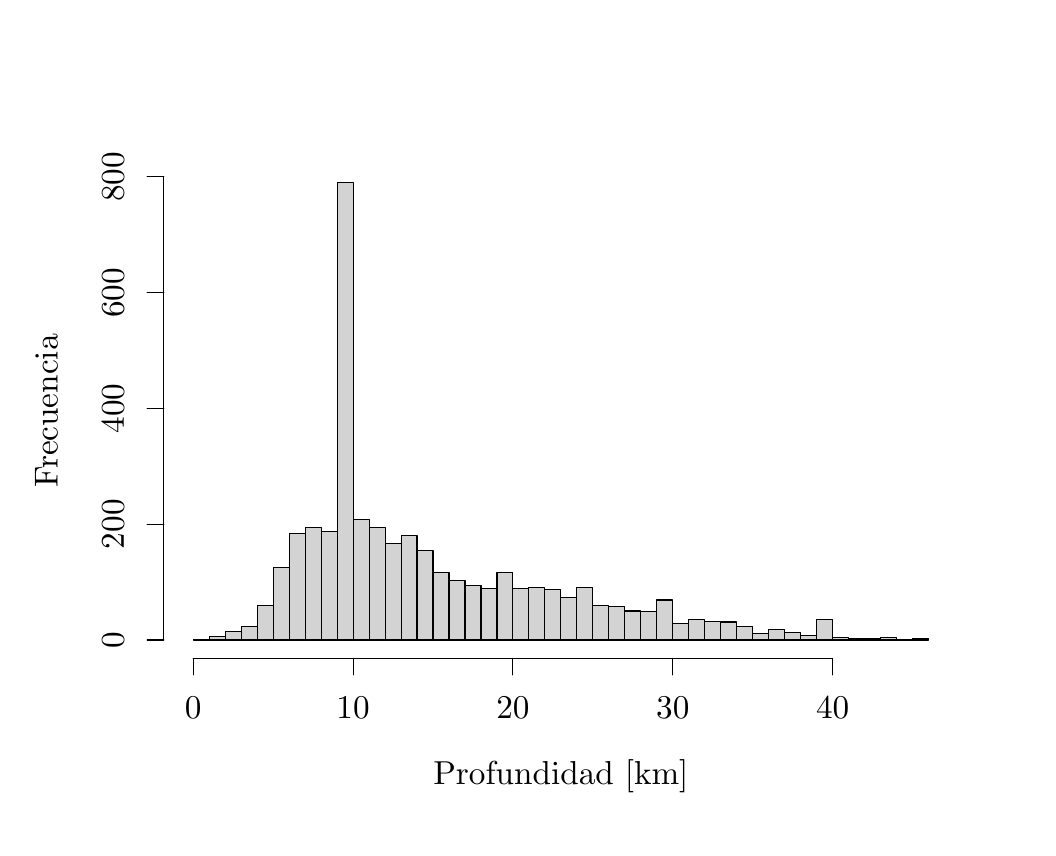
\begin{tikzpicture}[x=1pt,y=1pt]
\definecolor{fillColor}{RGB}{255,255,255}
\path[use as bounding box,fill=fillColor,fill opacity=0.00] (0,0) rectangle (361.35,289.08);
\begin{scope}
\path[clip] (  0.00,  0.00) rectangle (361.35,289.08);
\definecolor{drawColor}{RGB}{0,0,0}

\node[text=drawColor,anchor=base,inner sep=0pt, outer sep=0pt, scale=  1.20] at (192.68, 15.60) {Profundidad [km]};

\node[text=drawColor,rotate= 90.00,anchor=base,inner sep=0pt, outer sep=0pt, scale=  1.20] at ( 10.80,150.54) {Frecuencia};
\end{scope}
\begin{scope}
\path[clip] (  0.00,  0.00) rectangle (361.35,289.08);
\definecolor{drawColor}{RGB}{0,0,0}

\path[draw=drawColor,line width= 0.4pt,line join=round,line cap=round] ( 59.83, 61.20) -- (290.87, 61.20);

\path[draw=drawColor,line width= 0.4pt,line join=round,line cap=round] ( 59.83, 61.20) -- ( 59.83, 55.20);

\path[draw=drawColor,line width= 0.4pt,line join=round,line cap=round] (117.59, 61.20) -- (117.59, 55.20);

\path[draw=drawColor,line width= 0.4pt,line join=round,line cap=round] (175.35, 61.20) -- (175.35, 55.20);

\path[draw=drawColor,line width= 0.4pt,line join=round,line cap=round] (233.11, 61.20) -- (233.11, 55.20);

\path[draw=drawColor,line width= 0.4pt,line join=round,line cap=round] (290.87, 61.20) -- (290.87, 55.20);

\node[text=drawColor,anchor=base,inner sep=0pt, outer sep=0pt, scale=  1.20] at ( 59.83, 39.60) {0};

\node[text=drawColor,anchor=base,inner sep=0pt, outer sep=0pt, scale=  1.20] at (117.59, 39.60) {10};

\node[text=drawColor,anchor=base,inner sep=0pt, outer sep=0pt, scale=  1.20] at (175.35, 39.60) {20};

\node[text=drawColor,anchor=base,inner sep=0pt, outer sep=0pt, scale=  1.20] at (233.11, 39.60) {30};

\node[text=drawColor,anchor=base,inner sep=0pt, outer sep=0pt, scale=  1.20] at (290.87, 39.60) {40};

\path[draw=drawColor,line width= 0.4pt,line join=round,line cap=round] ( 49.20, 67.82) -- ( 49.20,235.14);

\path[draw=drawColor,line width= 0.4pt,line join=round,line cap=round] ( 49.20, 67.82) -- ( 43.20, 67.82);

\path[draw=drawColor,line width= 0.4pt,line join=round,line cap=round] ( 49.20,109.65) -- ( 43.20,109.65);

\path[draw=drawColor,line width= 0.4pt,line join=round,line cap=round] ( 49.20,151.48) -- ( 43.20,151.48);

\path[draw=drawColor,line width= 0.4pt,line join=round,line cap=round] ( 49.20,193.31) -- ( 43.20,193.31);

\path[draw=drawColor,line width= 0.4pt,line join=round,line cap=round] ( 49.20,235.14) -- ( 43.20,235.14);

\node[text=drawColor,rotate= 90.00,anchor=base,inner sep=0pt, outer sep=0pt, scale=  1.20] at ( 34.80, 67.82) {0};

\node[text=drawColor,rotate= 90.00,anchor=base,inner sep=0pt, outer sep=0pt, scale=  1.20] at ( 34.80,109.65) {200};

\node[text=drawColor,rotate= 90.00,anchor=base,inner sep=0pt, outer sep=0pt, scale=  1.20] at ( 34.80,151.48) {400};

\node[text=drawColor,rotate= 90.00,anchor=base,inner sep=0pt, outer sep=0pt, scale=  1.20] at ( 34.80,193.31) {600};

\node[text=drawColor,rotate= 90.00,anchor=base,inner sep=0pt, outer sep=0pt, scale=  1.20] at ( 34.80,235.14) {800};
\end{scope}
\begin{scope}
\path[clip] ( 49.20, 61.20) rectangle (336.15,239.88);
\definecolor{drawColor}{RGB}{0,0,0}
\definecolor{fillColor}{RGB}{211,211,211}

\path[draw=drawColor,line width= 0.4pt,line join=round,line cap=round,fill=fillColor] ( 59.83, 67.82) rectangle ( 65.60, 68.03);

\path[draw=drawColor,line width= 0.4pt,line join=round,line cap=round,fill=fillColor] ( 65.60, 67.82) rectangle ( 71.38, 69.07);

\path[draw=drawColor,line width= 0.4pt,line join=round,line cap=round,fill=fillColor] ( 71.38, 67.82) rectangle ( 77.16, 70.96);

\path[draw=drawColor,line width= 0.4pt,line join=round,line cap=round,fill=fillColor] ( 77.16, 67.82) rectangle ( 82.93, 72.84);

\path[draw=drawColor,line width= 0.4pt,line join=round,line cap=round,fill=fillColor] ( 82.93, 67.82) rectangle ( 88.71, 80.16);

\path[draw=drawColor,line width= 0.4pt,line join=round,line cap=round,fill=fillColor] ( 88.71, 67.82) rectangle ( 94.48, 93.96);

\path[draw=drawColor,line width= 0.4pt,line join=round,line cap=round,fill=fillColor] ( 94.48, 67.82) rectangle (100.26,106.30);

\path[draw=drawColor,line width= 0.4pt,line join=round,line cap=round,fill=fillColor] (100.26, 67.82) rectangle (106.04,108.39);

\path[draw=drawColor,line width= 0.4pt,line join=round,line cap=round,fill=fillColor] (106.04, 67.82) rectangle (111.81,106.93);

\path[draw=drawColor,line width= 0.4pt,line join=round,line cap=round,fill=fillColor] (111.81, 67.82) rectangle (117.59,233.26);

\path[draw=drawColor,line width= 0.4pt,line join=round,line cap=round,fill=fillColor] (117.59, 67.82) rectangle (123.36,111.32);

\path[draw=drawColor,line width= 0.4pt,line join=round,line cap=round,fill=fillColor] (123.36, 67.82) rectangle (129.14,108.39);

\path[draw=drawColor,line width= 0.4pt,line join=round,line cap=round,fill=fillColor] (129.14, 67.82) rectangle (134.92,102.54);

\path[draw=drawColor,line width= 0.4pt,line join=round,line cap=round,fill=fillColor] (134.92, 67.82) rectangle (140.69,105.47);

\path[draw=drawColor,line width= 0.4pt,line join=round,line cap=round,fill=fillColor] (140.69, 67.82) rectangle (146.47,100.03);

\path[draw=drawColor,line width= 0.4pt,line join=round,line cap=round,fill=fillColor] (146.47, 67.82) rectangle (152.24, 92.29);

\path[draw=drawColor,line width= 0.4pt,line join=round,line cap=round,fill=fillColor] (152.24, 67.82) rectangle (158.02, 89.36);

\path[draw=drawColor,line width= 0.4pt,line join=round,line cap=round,fill=fillColor] (158.02, 67.82) rectangle (163.80, 87.48);

\path[draw=drawColor,line width= 0.4pt,line join=round,line cap=round,fill=fillColor] (163.80, 67.82) rectangle (169.57, 86.43);

\path[draw=drawColor,line width= 0.4pt,line join=round,line cap=round,fill=fillColor] (169.57, 67.82) rectangle (175.35, 92.29);

\path[draw=drawColor,line width= 0.4pt,line join=round,line cap=round,fill=fillColor] (175.35, 67.82) rectangle (181.12, 86.43);

\path[draw=drawColor,line width= 0.4pt,line join=round,line cap=round,fill=fillColor] (181.12, 67.82) rectangle (186.90, 86.64);

\path[draw=drawColor,line width= 0.4pt,line join=round,line cap=round,fill=fillColor] (186.90, 67.82) rectangle (192.68, 86.22);

\path[draw=drawColor,line width= 0.4pt,line join=round,line cap=round,fill=fillColor] (192.68, 67.82) rectangle (198.45, 83.09);

\path[draw=drawColor,line width= 0.4pt,line join=round,line cap=round,fill=fillColor] (198.45, 67.82) rectangle (204.23, 86.64);

\path[draw=drawColor,line width= 0.4pt,line join=round,line cap=round,fill=fillColor] (204.23, 67.82) rectangle (210.00, 80.37);

\path[draw=drawColor,line width= 0.4pt,line join=round,line cap=round,fill=fillColor] (210.00, 67.82) rectangle (215.78, 79.95);

\path[draw=drawColor,line width= 0.4pt,line join=round,line cap=round,fill=fillColor] (215.78, 67.82) rectangle (221.55, 78.28);

\path[draw=drawColor,line width= 0.4pt,line join=round,line cap=round,fill=fillColor] (221.55, 67.82) rectangle (227.33, 78.07);

\path[draw=drawColor,line width= 0.4pt,line join=round,line cap=round,fill=fillColor] (227.33, 67.82) rectangle (233.11, 82.25);

\path[draw=drawColor,line width= 0.4pt,line join=round,line cap=round,fill=fillColor] (233.11, 67.82) rectangle (238.88, 73.88);

\path[draw=drawColor,line width= 0.4pt,line join=round,line cap=round,fill=fillColor] (238.88, 67.82) rectangle (244.66, 75.14);

\path[draw=drawColor,line width= 0.4pt,line join=round,line cap=round,fill=fillColor] (244.66, 67.82) rectangle (250.43, 74.51);

\path[draw=drawColor,line width= 0.4pt,line join=round,line cap=round,fill=fillColor] (250.43, 67.82) rectangle (256.21, 74.30);

\path[draw=drawColor,line width= 0.4pt,line join=round,line cap=round,fill=fillColor] (256.21, 67.82) rectangle (261.99, 72.84);

\path[draw=drawColor,line width= 0.4pt,line join=round,line cap=round,fill=fillColor] (261.99, 67.82) rectangle (267.76, 70.12);

\path[draw=drawColor,line width= 0.4pt,line join=round,line cap=round,fill=fillColor] (267.76, 67.82) rectangle (273.54, 71.58);

\path[draw=drawColor,line width= 0.4pt,line join=round,line cap=round,fill=fillColor] (273.54, 67.82) rectangle (279.31, 70.54);

\path[draw=drawColor,line width= 0.4pt,line join=round,line cap=round,fill=fillColor] (279.31, 67.82) rectangle (285.09, 69.49);

\path[draw=drawColor,line width= 0.4pt,line join=round,line cap=round,fill=fillColor] (285.09, 67.82) rectangle (290.87, 75.35);

\path[draw=drawColor,line width= 0.4pt,line join=round,line cap=round,fill=fillColor] (290.87, 67.82) rectangle (296.64, 68.86);

\path[draw=drawColor,line width= 0.4pt,line join=round,line cap=round,fill=fillColor] (296.64, 67.82) rectangle (302.42, 68.24);

\path[draw=drawColor,line width= 0.4pt,line join=round,line cap=round,fill=fillColor] (302.42, 67.82) rectangle (308.19, 68.24);

\path[draw=drawColor,line width= 0.4pt,line join=round,line cap=round,fill=fillColor] (308.19, 67.82) rectangle (313.97, 68.65);

\path[draw=drawColor,line width= 0.4pt,line join=round,line cap=round,fill=fillColor] (313.97, 67.82) rectangle (319.75, 68.03);

\path[draw=drawColor,line width= 0.4pt,line join=round,line cap=round,fill=fillColor] (319.75, 67.82) rectangle (325.52, 68.24);
\end{scope}
\end{tikzpicture}
